%        File: crs.tex
%     Created: jeu. juin 07 10:00  2018 C
% Last Change: jeu. juin 07 10:00  2018 C
%
\documentclass[a4paper]{report}
\usepackage{amsmath}
\usepackage[utf8]{inputenc}
\usepackage{array}
\usepackage[titlenumbered, ruled]{algorithm2e}
\usepackage{xr}
\externaldocument{survey}
\usepackage{booktabs}
\SetKwRepeat{Do}{do}{while}

\usepackage{graphicx}
%\usepackage{subcaption}
%\captionsetup[subfigure]{font=scriptsize}
\DeclareGraphicsExtensions{.pdf,.png,.jpeg,.jpg}
\graphicspath{{./img/}}

\begin{document}
\chapter{Collaborative Reconstruction Network}

The Collaborative Clustering paradigm is based on the prerequisite that each view has to contain a set of common individuals (described by different sets of features for the horizontal case) as big as possible to allow to exchange information. However, the individuals which are not common to all the views are not used in this paradigm. We introduce in this section a method which use these remaining data to construct an approximation of the individual in the views where it is missing.\\

\section{Context}
\label{sec:crs_context}

This method may be used to solve problem such as cold start in some cases. For example, if the scores of a player are known for a certain amount of games, its predicted scores could be approximated for a game he hasn't played yet. This approximation could then be used to improve match-making (the action to group people supposedly balanced teams before entering a game) or even to recommend a new game to this player. This would typically be impossible without prior information of the player, but the system presented here takes the information from external views and use it to build an approximation of the seeked information.\\

This problem of predicting missing values based on existing ones is not new, and has already been extensively studied in fields such as recommendation (in~\cite{chen2014hybrid},~\cite{hallinan2016recommended},~\cite{wang2015friendbook} and~\cite{covington2016deep} for example) or such as collaborative filtering~\cite{koren2015advances}. However, what we present here is a reconsutruction system with an additionnal constraint: a view should not have access to original data from its external peers.\\

This constraint has naturally appeared because of the growing concern of people regarding their private data and the use that is made of them. The fast growth of social networks such as Facebook and Twitter or even the targeted advertising performed by Google are examples of generation and use that can be made of people everydays data. Based on this concern, our method shares the information without communication of any original data between views. This is based on the anonymization of each original database using an autoencoder (see Section~\ref{sec:nn} for further details). Using this method, the information which is transfered between views do not permit to recover the original data, while being usable for further analysis (see Section~\ref{sec:archi} for a detailed architecture of the system). In the next is presented a quick summary of what is a Neural Network, the machine learning algorithm on which is based the Collaborative Reconstruction System presented here.


\section{Neural Networks}
\label{sec:nn}

\subsection{Introduction}

Neural Networks are a specific kind of Machine Learning algorithm based on an analogy of the interaction of the neurons in a human brain. Their history has known many steps the most known being the presentation of the perceptron (a.k.a.\ a neuron) by Rosenblatt in 1958~\cite{rosenblatt1958perceptron}, the use of the backpropagation algorithm by Werbos in 1975~\cite{werbos1974beyond} and the presentation of the deep beliefs networks by Hinton in 2006~\cite{hinton2006fast}. The original version has been modified to produce several types of neural networks, depending on the aim to achieve. The two most famous being Convolutional Neural Network~\cite{krizhevsky2012imagenet} to perform image analysis and the Recurrent Neural Network~\cite{mikolov2010recurrent} which are used to analyze temporal data. In this thesis, we are only interested in the Multi Layer Perceptron. The following sections briefly sum up the principal components of a Multi Layer Perceptron (MLP). 

\subsection{A neuron}

A MLP is made of several layers of several neurons (see Figure~\ref{fig:neuron}), each having a set a parameters which are trained during the MLP learning. To get the ouput of a neuron, each feature of the input vector is weighted by a parameter of the neuron, before being summed and put in an activation function to get the final output. Regarding the activation function, the first one which has been used is the sigmoid function, which definition can be found at Equation~\ref{eq:sigmoid}. There are many different activation functions which can be used, however the one which tends to be the most commonly met in recent research work is the Rectified Linear Unit (ReLU), which definition is simply $ReLU(x) = \max(0, x)$. The activation function being known. The backpropagation algorithm is applied to train the weighting coefficients of the neuron.


    \begin{figure}[h]
        \centering
        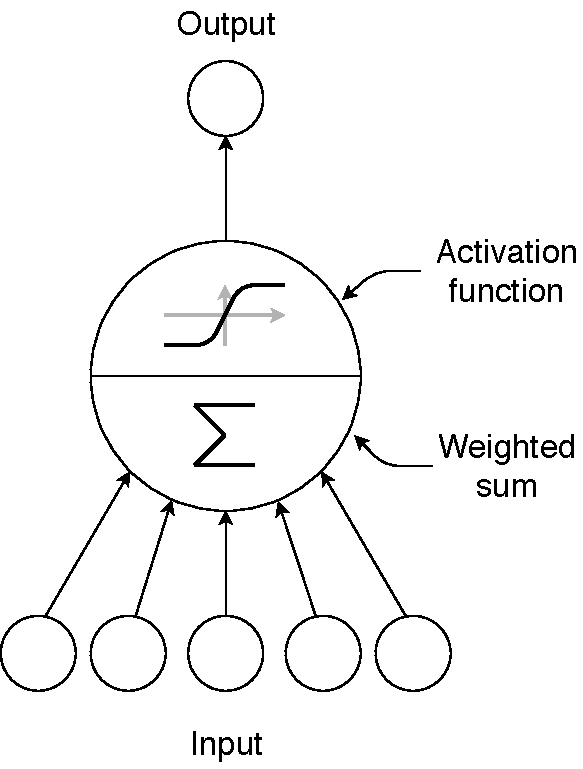
\includegraphics[scale=.6]{perceptron}
        \caption{A single neuron. Each input $x_i$ is weighted by a parameter $w_i$ before being summed and put in an activation function. The output from this funtion corresponds to the output of the neuron.}
\label{fig:neuron}
    \end{figure}

    \begin{equation}
        sigmoid(x) = \frac{1}{1 + \exp(-x)} = \frac{\exp(x)}{1 + \exp(x)}
        \label{eq:sigmoid}
    \end{equation}

    \subsection{The backpropagation method}
    The backpropagation method consists in the the propagation of the gradient of the error between the ouput of the MLP and what is expected from the output to the input of the system, hence the term backpropagation. The main equation of the gradient descent is the one presented in Equation~\ref{eq:gd_main}, with $w$ being the parameter to optimize, and $E$ the error function depending on $w$. The minus symbol represents the idea that, when using this method, one tries to achieve the lowest point of the error function, as graphically represented on Figure~\ref{fig:gd}. 

\begin{equation}
    w_{new} = w_{old} - \varepsilon \times \frac{\partial E}{\partial w}
    \label{eq:gd_main}
\end{equation}

    \begin{figure}[h]
        \centering
        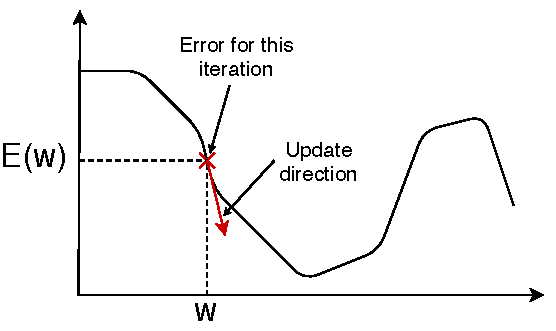
\includegraphics{gd}
        \caption{One step of gradient descent. The red cross is the current point, while the red arrow represents the direction in which the parameter has to be updated to lower the error.}
\label{fig:gd}
    \end{figure}

    The main difficulty of the update of the parameter using Equation~\ref{eq:gd_main} is to compute the value of the partial derivative of the error function $E$. This is achieved using the partial derivative composition property considering that the $E$ function can be written as follows:

    \begin{equation}
        E\left(x_{target}, x_{output}, W\right) = l\left(x_{target}, f\left(\sum_{i=1}^I w_i x_i\right)\right)
        \label{eq:error_function}
    \end{equation}

    With $l$ a loss function such as the $l_2$-norm, $f$ the activation function of the neuron, $x_i$ the $i$-th value of the input (with a total of $I$ input) and $w_i$ the corresponding weight of the neuron. For clarity of the equation, the following notation will be used:

    \begin{equation}
        a_i = \sum_{i=1}^I w_i x_i
        \label{eq:weighted_sum}
    \end{equation}

    This allows to express the partial derivative of $E$ in the following way:

    \begin{equation}
        \frac{\partial E}{\partial w} = \frac{\partial E}{\partial f\left( a_i\right)} \frac{\partial f(a_i)}{\partial a_i}\frac{\partial a_i}{\partial w_i} = \frac{\partial E}{\partial f\left( a_i\right)} \frac{\partial f(a_i)}{\partial a_i} x_i
        \label{eq:partial_composition}
    \end{equation}

    Equation~\ref{eq:partial_composition} being generic, it can be used with any combination of loss and activation functions. The same composition rule is also used when dealing with several layers of neurons, but in this case the partial derivate of $a_i$ by $w_i$ has to be composed again in order to ``reach'' the parameter $w_i$ in the following layer.\\

    Knowing this method, the learning of a MLP is performed by iteratively applying Equation~\ref{eq:gd_main} to all the parameters of the network until the norm of the gradient is small enough to be considered negligeable. In the following Section are presented the two kinds of Neural Networks which are trained by this method and which are used in the CRS.\@

    \subsection{MLP and Autoencoder}

    The term MLP designates the supervised Neural Network algorithm which makes possible to learn a regression between the input and the output. This definition implies that the input and the output have to be different. A special kind of Neural Networks, presented in~\cite{vincent2008extracting}, uses the input of the system as its output. They are called Autoencoders, because the intermediate layers of the networks, and more specifically their activations, can be used as codes to represent the input individuals. A graphical representation of both the MLP and the Autoencoder are presented on Figure~\ref{fig:mlp_ae}.\\

    \begin{figure}[h]
        \centering
        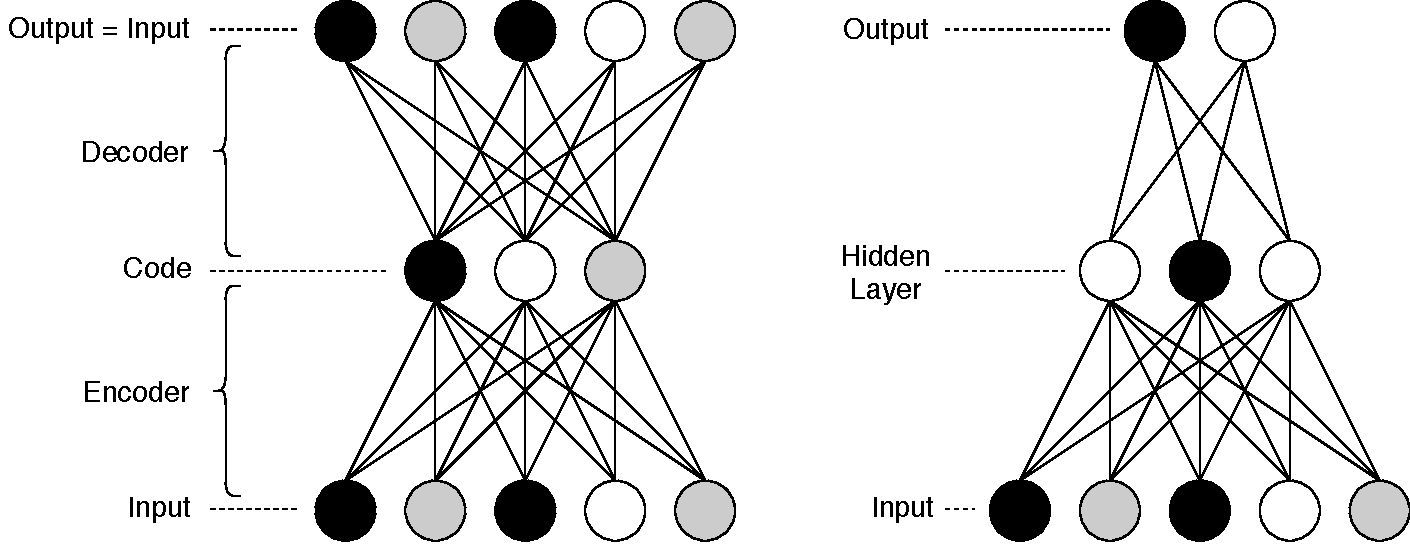
\includegraphics[scale=.5]{mlp_ae}
        \caption{An Autoencoder (left) and a Multi-Layer Perceptron (right). The intensity of the grey in each neuron symbolizes its activation.}
\label{fig:mlp_ae}
    \end{figure}
    
    This kind of network is composed of two subnetworks trained together: the one between the input and the hidden layer used as code called the encoder, and the one between the code layer and the output called the decoder. While it has not been strictly demonstrate, one of the advantage of this kind of network is to make the coded version of a sample undecryptable without the access to the decoder network.\\

    The use of these two kinds of network in the Collaborative Reconstruction system is detailed in Section~\ref{sec:archi}.

\section{Architecture}
\label{sec:archi}

To recall Section~\ref{sec:crs_context}, the Collaborative Reconstruction System is defined through 3 different axes:

\begin{itemize}
    \item The reconstruction of missing data\dots
    \item \dots in a collaborative context\dots
    \item \dots with a privacy constraint.
\end{itemize}

The design of the method has been defined following these three points. Thus, the global architecture of a CRS is made of 3 main components:

\begin{itemize}
    \item A set of Autoencoders to encode data available in each view. This ensures that no original data will be shared among the views.
    \item A set of Multi-Layer Perceptrons to decode the data got from each external view.
    \item A method which combines the representations received from each external view, here called the Masked Weighting Method.
\end{itemize}

This Section presents the use of each component and how they are linked together. A graphical representation of the whole system can be found on Figure~\ref{fig:crs}.

\begin{figure}[h]
    \centering
    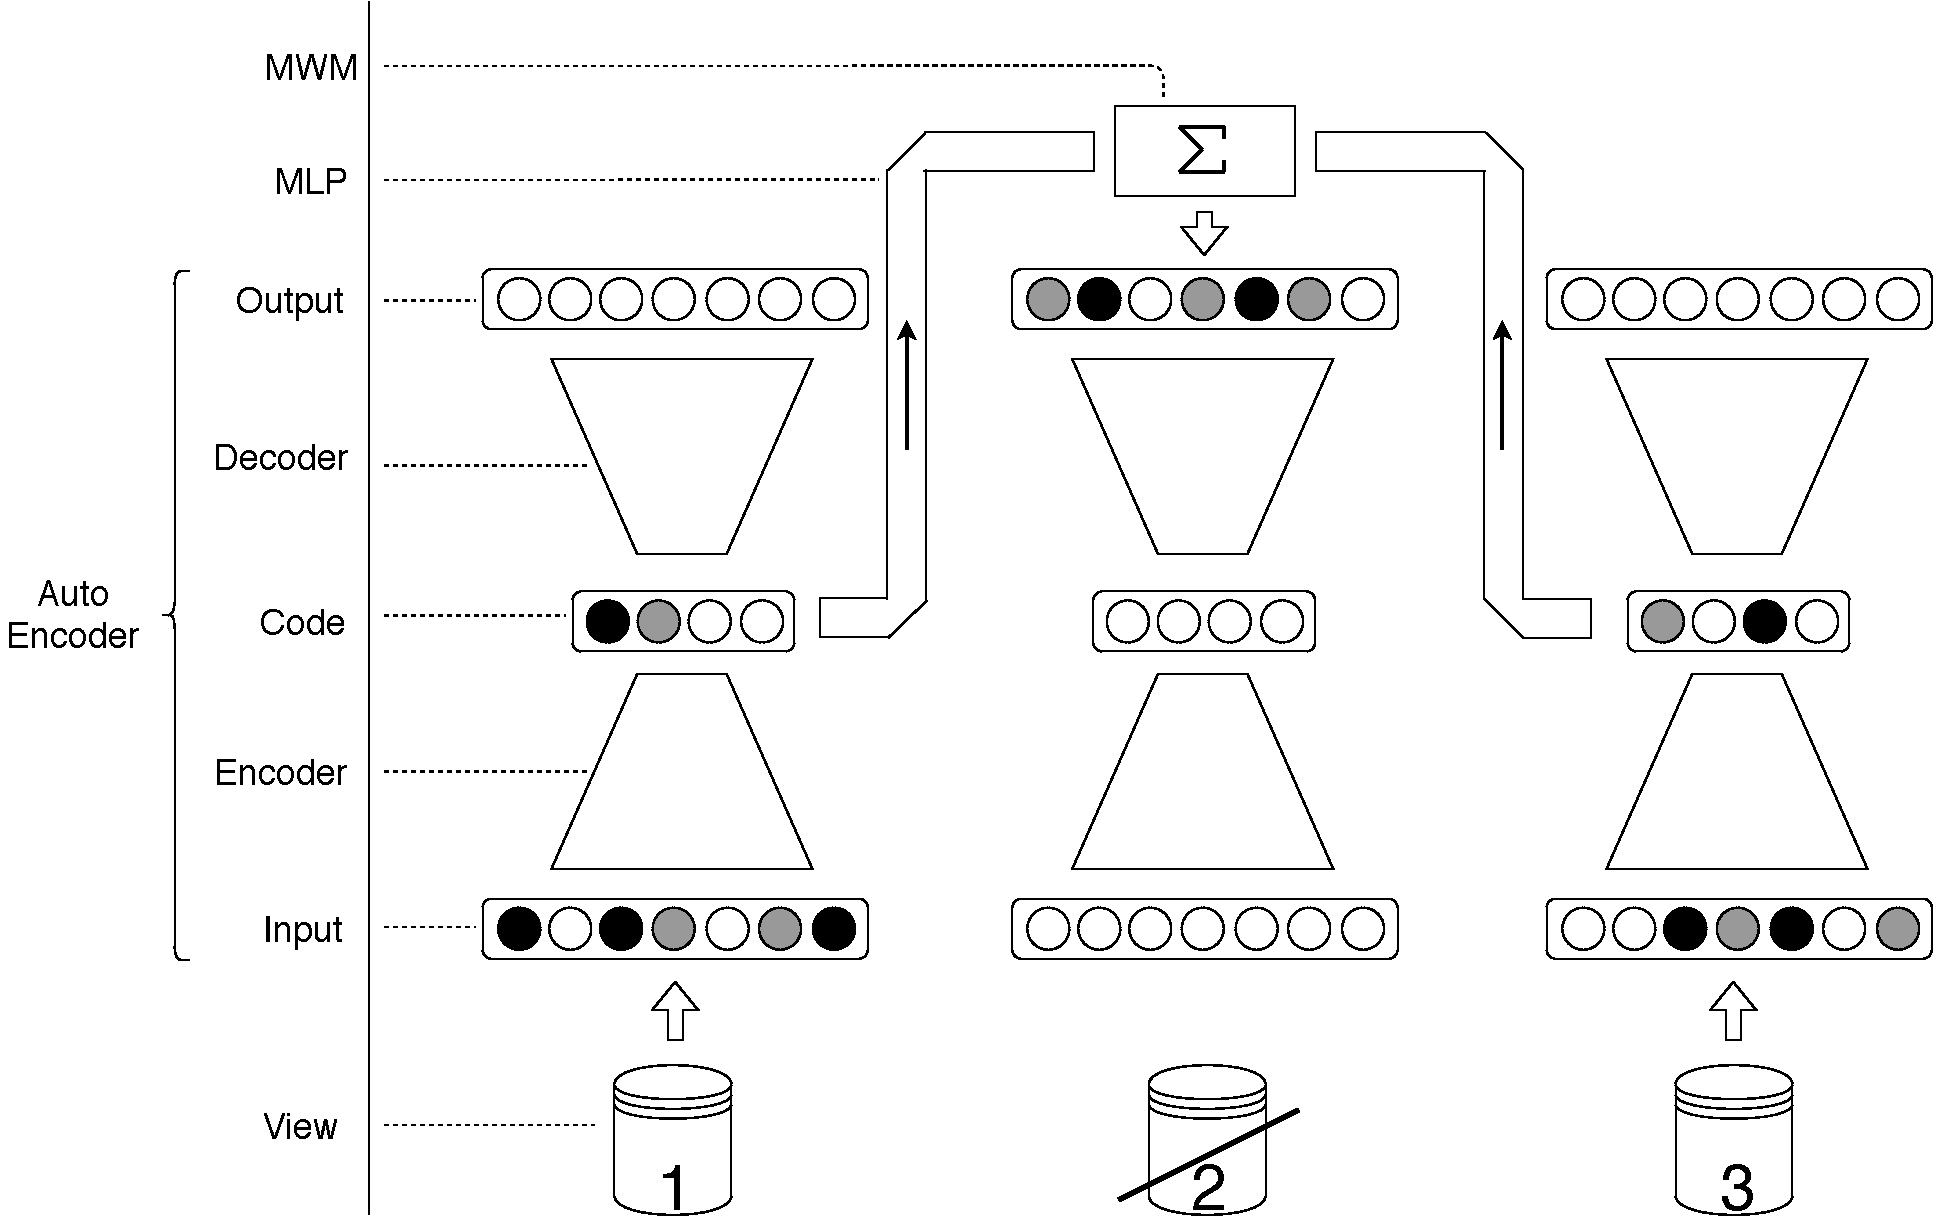
\includegraphics[scale=.25]{base_system}
    \caption{Architecture of a Collaborative Reconstruction System with 3 views. In this example, an individual is missing in the second view.}
\label{fig:crs}
\end{figure}

This system is based on the horizontal Collaborative Clustering (see Section~\ref{sec:cc_hor_ver})

    \subsection{One Autoencoder per view}

    To ensure that no view can access the original data from an external view, one autoencoder per view is trained in order to cypher the original data. The advantage of this method is that the data is encoded under the form of a scalar vector which can be used for further applications. The architecture of the autoencoders does not have to be the same for all the views. The important point is to ensure that the representation makes possible to get a good reconstruction of the individual at the output. In other words, one wants to ensure that the code is defined in such a way that it allows to retrieve the original data: the difference of information between the individual and its coded version should be as small as possible. This latter point is important because if it is not verified, the external reconstruction based on the defective coded version may be greatly harmed.\\

    However, in order to make it possible for a Link (see Section~\ref{sec:crs_link}) to reconstruct an individual, the size of the code should also be as small as possible. The smaller the size of the code, the easier the training of the associated Link.\\

    The first step of the training of the CRS is to train one Autoencoder per view and to encode each original dataset using these latter. At the end of this step, $N$ encoded datasets are available for the next step. From now, the original dataset of the $i$-th view is called $V_i$ and the subset of $V_i$ which only contains individuals which also have a representation in the $j$-th view is called $V_{i|j}$. This clarification of notation is important because during in the following Section, the training of the Link relies entirely on the subset of each dataset with common individuals.

    \subsection{Links to get the external reconstructions}

    When each original dataset has been encoded, it is possible to start the training of the MLP which are responsible of the reconstruction of the missing individual. In the context of this system, the MLP are called the Links to represent the fact that their role is to draw a link between each pair of views. The training process is the same as the one described in Section~\ref{sec:nn}. However, the datasets used as input and output have to be precised: because of its role, a Link needs to have each time two representations of the same individual, namely the one coded by the autoencoder in the external view, and the original one from the output view. This is the context previously defind in~\ref{sec:cc_hor_ver} about the Horizontal Collaborative Clustering. A graphical representation of the learning process of a Link is displayed on Figure~\ref{fig:crs_link}.\\
    
    It has to be noted that, because of the privacy constraint, the learning is supposed to be launched in the view with the original output data. For example, in a problem with 3 different views, the Link trained with the encoded database of the first view and the original database of the second view is supposed to be accessible only by actors from the second views, because only them are supposed to have access to the original data from the second view. Moreover, during the training, when looking at the error produced by the network, the reconstruction based on the coded version of an individiual $x_i$ has to be compared with the version of $x_i$ available in the output view.

    \vspace{0.8cm}

    \begin{figure}[h]
        \centering
        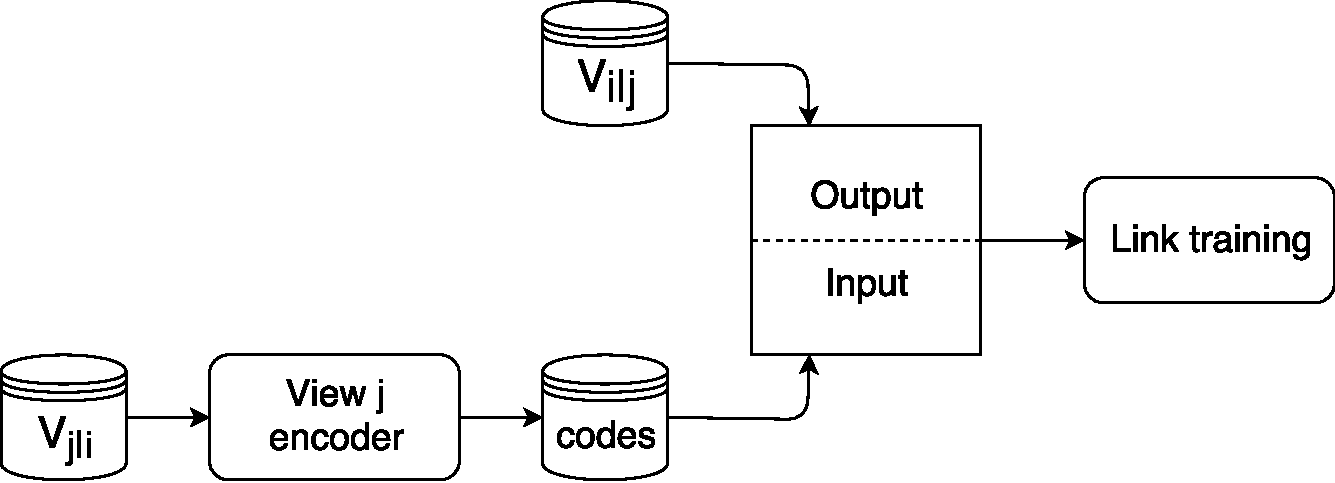
\includegraphics[scale=.5]{links}
        \caption{Training process of a Link. Each external dataset is encoded and is feeded as input to the Link, while the original dataset is used as the output.}
\label{fig:crs_link}
    \end{figure}

    Here again, the architectures of the Links are independent one from another, the only obvious constraints being that the input layer has the same number of neurons than the code it has to decode and that the output layer has the same number of neurons than the dimension of the output space.\\

    When a view $i$ has access to the $N-1$ Links trained with the $N-1$ respective external datasets, it has access to $N-1$ representations of a potentially missing individual. In the next Section is presented a weighting method which aim is to find the best combination of these $N-1$ individuals in order to get the best final reconstruction.

    \subsection{The Masked Weighting Method}

    \subsection{The Reconstruction Process}

    \subsection{The system Modularity}

\label{sec:crs_link}

\section{Experiments}
\label{sec:exp}

\section{Limitations}
\label{sec:limit}

\section{Perspectives}
\label{sec:perspectives}



    \bibliographystyle{plain}
    \bibliography{bib.bib}
\end{document}


